\documentclass[a4paper]{report}
% Some basic packages
\usepackage[utf8]{inputenc}
\usepackage[T1]{fontenc}
\usepackage{textcomp}
\usepackage[english]{babel}
\usepackage{url}
\usepackage{graphicx}
\usepackage{float}
\usepackage{booktabs}
\usepackage{enumitem}

\pdfminorversion=7

% Don't indent paragraphs, leave some space between them
\usepackage{parskip}

% Hide page number when page is empty
\usepackage{emptypage}
\usepackage{subcaption}
\usepackage{multicol}
\usepackage{xcolor}

% Other font I sometimes use.
% \usepackage{cmbright}

% Math stuff
\usepackage{amsmath, amsfonts, mathtools, amsthm, amssymb}
% Fancy script capitals
\usepackage{mathrsfs}
\usepackage{cancel}
% Bold math
\usepackage{bm}
% Some shortcuts
\newcommand\N{\ensuremath{\mathbb{N}}}
\newcommand\R{\ensuremath{\mathbb{R}}}
\newcommand\Z{\ensuremath{\mathbb{Z}}}
\renewcommand\O{\ensuremath{\emptyset}}
\newcommand\Q{\ensuremath{\mathbb{Q}}}
\newcommand\C{\ensuremath{\mathbb{C}}}
\renewcommand\L{\ensuremath{\mathcal{L}}}

% Package for Petri Net drawing
\usepackage[version=0.96]{pgf}
\usepackage{tikz}
\usetikzlibrary{arrows,shapes,automata,petri}
\usepackage{tikzit}
\input{petri_nets_style.tikzstyles}

% Easily typeset systems of equations (French package)
\usepackage{systeme}

% Put x \to \infty below \lim
\let\svlim\lim\def\lim{\svlim\limits}

%Make implies and impliedby shorter
\let\implies\Rightarrow
\let\impliedby\Leftarrow
\let\iff\Leftrightarrow
\let\epsilon\varepsilon

% Add \contra symbol to denote contradiction
\usepackage{stmaryrd} % for \lightning
\newcommand\contra{\scalebox{1.5}{$\lightning$}}

% \let\phi\varphi

% Command for short corrections
% Usage: 1+1=\correct{3}{2}

\definecolor{correct}{HTML}{009900}
\newcommand\correct[2]{\ensuremath{\:}{\color{red}{#1}}\ensuremath{\to }{\color{correct}{#2}}\ensuremath{\:}}
\newcommand\green[1]{{\color{correct}{#1}}}

% horizontal rule
\newcommand\hr{
    \noindent\rule[0.5ex]{\linewidth}{0.5pt}
}

% hide parts
\newcommand\hide[1]{}

% si unitx
\usepackage{siunitx}
\sisetup{locale = FR}

% Environments
\makeatother
% For box around Definition, Theorem, \ldots
\usepackage{mdframed}
\mdfsetup{skipabove=1em,skipbelow=0em}
\theoremstyle{definition}
\newmdtheoremenv[nobreak=true]{definitie}{Definitie}
\newmdtheoremenv[nobreak=true]{eigenschap}{Eigenschap}
\newmdtheoremenv[nobreak=true]{gevolg}{Gevolg}
\newmdtheoremenv[nobreak=true]{lemma}{Lemma}
\newmdtheoremenv[nobreak=true]{propositie}{Propositie}
\newmdtheoremenv[nobreak=true]{stelling}{Stelling}
\newmdtheoremenv[nobreak=true]{wet}{Wet}
\newmdtheoremenv[nobreak=true]{postulaat}{Postulaat}
\newmdtheoremenv{conclusie}{Conclusie}
\newmdtheoremenv{toemaatje}{Toemaatje}
\newmdtheoremenv{vermoeden}{Vermoeden}
\newtheorem*{herhaling}{Herhaling}
\newtheorem*{intermezzo}{Intermezzo}
\newtheorem*{notatie}{Notatie}
\newtheorem*{observatie}{Observatie}
\newtheorem*{exe}{Exercise}
\newtheorem*{opmerking}{Opmerking}
\newtheorem*{praktisch}{Praktisch}
\newtheorem*{probleem}{Probleem}
\newtheorem*{terminologie}{Terminologie}
\newtheorem*{toepassing}{Toepassing}
\newtheorem*{uovt}{UOVT}
\newtheorem*{vb}{Voorbeeld}
\newtheorem*{vraag}{Vraag}

\newmdtheoremenv[nobreak=true]{definition}{Definition}
\newtheorem*{eg}{Example}
\newtheorem*{notation}{Notation}
\newtheorem*{previouslyseen}{As previously seen}
\newtheorem*{remark}{Remark}
\newtheorem*{note}{Note}
\newtheorem*{problem}{Problem}
\newtheorem*{observe}{Observe}
\newtheorem*{property}{Property}
\newtheorem*{intuition}{Intuition}
\newmdtheoremenv[nobreak=true]{prop}{Proposition}
\newmdtheoremenv[nobreak=true]{theorem}{Theorem}
\newmdtheoremenv[nobreak=true]{corollary}{Corollary}

% End example and intermezzo environments with a small diamond (just like proof
% environments end with a small square)
\usepackage{etoolbox}
\AtEndEnvironment{vb}{\null\hfill$\diamond$}%
\AtEndEnvironment{intermezzo}{\null\hfill$\diamond$}%
% \AtEndEnvironment{opmerking}{\null\hfill$\diamond$}%

% Fix some spacing
% http://tex.stackexchange.com/questions/22119/how-can-i-change-the-spacing-before-theorems-with-amsthm
\makeatletter
\def\thm@space@setup{%
  \thm@preskip=\parskip \thm@postskip=0pt
}


% Exercise 
% Usage:
% \exercise{5}
% \subexercise{1}
% \subexercise{2}
% \subexercise{3}
% gives
% Exercise 5
%   Exercise 5.1
%   Exercise 5.2
%   Exercise 5.3
\newcommand{\exercise}[1]{%
    \def\@exercise{#1}%
    \subsection*{Exercise #1}
}

\newcommand{\subexercise}[1]{%
    \subsubsection*{Exercise \@exercise.#1}
}


% \lecture starts a new lecture (les in dutch)
%
% Usage:
% \lecture{1}{di 12 feb 2019 16:00}{Inleiding}
%
% This adds a section heading with the number / title of the lecture and a
% margin paragraph with the date.

% I use \dateparts here to hide the year (2019). This way, I can easily parse
% the date of each lecture unambiguously while still having a human-friendly
% short format printed to the pdf.

\usepackage{xifthen}
\def\testdateparts#1{\dateparts#1\relax}
\def\dateparts#1 #2 #3 #4 #5\relax{
    \marginpar{\small\textsf{\mbox{#1 #2 #3 #5}}}
}

\def\@lecture{}%
\newcommand{\lecture}[3]{
    \ifthenelse{\isempty{#3}}{%
        \def\@lecture{Lecture #1}%
    }{%
        \def\@lecture{Lecture #1: #3}%
    }%
    \subsection*{\@lecture}
    \marginpar{\small\textsf{\mbox{#2}}}
}



% These are the fancy headers
\usepackage{fancyhdr}
\pagestyle{fancy}

% LE: left even
% RO: right odd
% CE, CO: center even, center odd
% My name for when I print my lecture notes to use for an open book exam.
% \fancyhead[LE,RO]{Gilles Castel}

\fancyhead[RO,LE]{\@lecture} % Right odd,  Left even
\fancyhead[RE,LO]{}          % Right even, Left odd

\fancyfoot[RO,LE]{\thepage}  % Right odd,  Left even
\fancyfoot[RE,LO]{}          % Right even, Left odd
\fancyfoot[C]{\leftmark}     % Center

\makeatother




% Todonotes and inline notes in fancy boxes
\usepackage{todonotes}
\usepackage{tcolorbox}

% Make boxes breakable
\tcbuselibrary{breakable}

% Verbetering is correction in Dutch
% Usage: 
% \begin{verbetering}
%     Lorem ipsum dolor sit amet, consetetur sadipscing elitr, sed diam nonumy eirmod
%     tempor invidunt ut labore et dolore magna aliquyam erat, sed diam voluptua. At
%     vero eos et accusam et justo duo dolores et ea rebum. Stet clita kasd gubergren,
%     no sea takimata sanctus est Lorem ipsum dolor sit amet.
% \end{verbetering}
\newenvironment{verbetering}{\begin{tcolorbox}[
    arc=0mm,
    colback=white,
    colframe=green!60!black,
    title=Opmerking,
    fonttitle=\sffamily,
    breakable
]}{\end{tcolorbox}}

% Noot is note in Dutch. Same as 'verbetering' but color of box is different
\newenvironment{noot}[1]{\begin{tcolorbox}[
    arc=0mm,
    colback=white,
    colframe=white!60!black,
    title=#1,
    fonttitle=\sffamily,
    breakable
]}{\end{tcolorbox}}




% Figure support as explained in my blog post.
\usepackage{import}
\usepackage{xifthen}
\usepackage{pdfpages}
\usepackage{transparent}
\newcommand{\incfig}[1]{%
    \def\svgwidth{\columnwidth}
    \import{./figures/}{#1.pdf_tex}
}

% Fix some stuff
% %http://tex.stackexchange.com/questions/76273/multiple-pdfs-with-page-group-included-in-a-single-page-warning
\pdfsuppresswarningpagegroup=1


% My name
\author{Bruno M. Pacheco}


\title{Advanced Process Mining - Exam Summary}

\begin{document}

\section*{Review of Fundamentals}

Transfer function representation: \[
    G(s) = \frac{K \Pi_i \left( s-s_i \right) }{s^{M}\Pi_j \left( s-s_j \right) }
\] in which $M$ is the \textbf{system type}, the measure of its complexity.

Second order system canonical form: \[
    G(s) = \frac{\omega^{2}_o}{s^{2} + 2\zeta\omega_o s + \omega^{2}_o}
\]. The step response is, given poles of the form \[
s = \omega_o\left( -\zeta \pm j\sqrt{1-\zeta^{2}}  \right) 
\] determined by:
\begin{itemize}
    \item $0\le \zeta < 1$ complex conjugate poles, underdamped;
    \item $\zeta = 0$ two conjugate poles on the imaginary axis, undamped;
    \item $\zeta > 1$ two different real poles, overdamped;
     \item $\zeta = 1$ one real pole, critically damped.
\end{itemize}

Phase margin can be computed as, approximately  \[
\varphi_m = 100\zeta
\].

Steady-state error:
\begin{align*}
    &\lim_{t \to \infty} e(t) = \lim_{s \to 0} sE(s) \\
    & \text{and } E(s) = \frac{1}{1+G(s)}U(s) 
.\end{align*}

\begin{description}
    \item[Perfect tracking] $\lim_{t \to \infty} e(t) = 0$, in which error is measured as the difference between reference and output;
\end{description}

\subsection*{Stability}

Real part of poles should be $<0$ :
\begin{itemize}
    \item In frequency domain: $F(s) = \frac{N(s)}{D(s)}$, the poles are the roots of $D(s) = 0$
    \item In state-space: $\dot{x}(t) = Ax(t) + Bu(t)$, poles are the roots of $det(\lambda I - A) = 0$
\end{itemize}

TODO: Nyquist plot, review criteria below!

Nyquist stability criteria: given $N$ clockwise encirclements (counterclockwise count as negative) of the point $-1+j0$, we can use \[
Z = N + P
\] in which Z are the closed-loop poles (zeros of the denominator) in the RHP and P are the open-loop poles in the RHP. This way, if we know the number of poles on the RHP of the open-loop TF (which usually are easy to calculate) and the Nyquist plot, we can find out how many poles in the RHP the closed-loop TF has.

In bode plots, gain margin is the magnitude $|G(j\omega)|$ where the phase angle is $-180º$, while phase margin is the difference, at null logarithmic gain, between the actual phase angle $f$ and $-180º$, that is,  $180 + f$.

\begin{figure}[H]
    \centering
    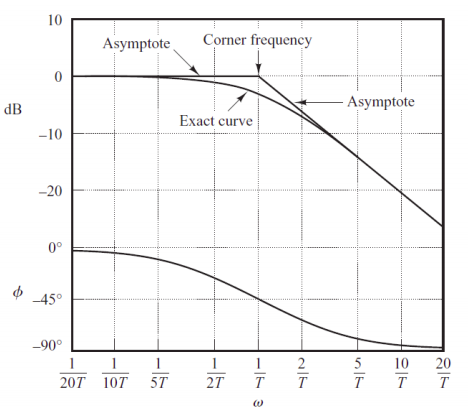
\includegraphics[width=0.6\textwidth]{bode_plot.png}
    \caption{Bode plot for unitary gain, single pole TF. If there is gain, add $20\log K$. Slope is 20 times the degree of the pole. Phase is -90º times the degree of the pole. Second degree adds an overshoot at the corner given by $\zeta$.}
    \label{fig:bode_plot-png}
\end{figure}

Ruth's stability criteria states that, given a polynomial like \[
\frac{1}{a_0s^{n}+a_1s^{n-1}+\ldots+a_n}
\] with $a_n \neq 0$, then, if any of the coefficients is zero or negative (unless they all are), \emph{at least one pole exists that has $\ge 0$ real part}.
 \subsection*{Controllers}

\begin{description}
    \item[P] $R(s) = K_p$
    \item[PI] $R(s) = K_p + \frac{K_I}{s}$
    \item[PID] $R(s) = K_p + \frac{K_I}{s} + K_D s$
\end{description}

\section*{Pole Placement}

State-space description is the minimum amount of information (differential equations) necessary to predict the behavior of the system.

General formulation: \[
\begin{cases}
    \dot{\bm{x}}(t) &= A\bm{x}(t) + B\bm{u}(t)\text{,  }\bm{x}(0) = \bm{x}_0 \\
    \bm{y}(t) &= C\bm{x}(t) + D\bm{u}(t) \\
\end{cases}
\] 

General solution: \[
    \bm{x}(t) = e^{At}\bm{x}_0 + \int_0^{t} e^{A\left( t-\tau \right) }B\bm{u}(\tau)d\tau
\] and in the frequency domain: \[
X(s) = (sI-A)^{-1}\bm{x}(0) + (sI-A)^{-1}BU(s)
\]. We call $e^{At}$ the \emph{transition matrix}.

\subsection*{Stability}

\textbf{If one eigenvalue of $A$ has real part positive, at least one variable grows exponentially.} The eigenvalues can be found from the characteristic equation \[
det\left( \lambda I - A \right) = 0
\].

\begin{definition}
    (Cayley-Hamilton) Given a square matrix $A$ and its characteristic polynomial defined as \[
    P(s) = det\left( \lambda I - A \right) = 0
    \] then, matrix $A$ is also a solution to the matrix equivalent of its polynomial, that is \[
    P(A) = 0
\]. \emph{This can be used to calculate higher powers of $A$ by isolating the highest degree of the polynomial}.
\end{definition}

\subsection*{Canonical forms}

Given a transfer function of the form \[
    G(s) = \frac{Y(s)}{U(s)} = \frac{b_ms^{m}+\ldots+b_1s + b_0}{s^{n}+a_{n-1}s^{n_1}+\ldots+a_0}\text{, }m<n
\] \emph{canonical forms} are processes to map into a state-space representation.

\subsubsection*{Controllable}

\begin{align*}
    &A = \begin{bmatrix}
	0 & 1 & 0 & \ldots & 0 \\ 
	0 & 0 & 1 & \ldots & 0 \\
	\vdots &  &  & \ddots & \vdots \\
	0 & 0 & 0 & \ldots & 1 \\
	-a_0 & -a_1 & -a_2 & \ldots & -a_{n-1}
	\end{bmatrix}; B = \bm{b} = \begin{bmatrix} 0 \\ \vdots \\ 0 \\ 1 \end{bmatrix} \\
	     &C = \bm{c}^{T} = \begin{bmatrix} (b_0 - b_na_0) & \ldots & (b_i - b_na_i) & \ldots & (b_{n-1} - b_na_{n-1}) \end{bmatrix} ; D = \bm{d} = \begin{bmatrix} b_n \end{bmatrix} 
.\end{align*}

\subsubsection*{Observable}

Dual to the controllable form:
\begin{align*}
    &A = A_{controllable}^{T}; B = \bm{c}_{controllable} \\
	     &C = \bm{b}_{controllable}^{T} ; D = \bm{d} = \begin{bmatrix} b_n \end{bmatrix} 
.\end{align*}

\subsubsection*{Diagonal or Jordan}

Based on the partial fractions expansion of the transfer function: \[
    G(s) = \frac{Y(s)}{U(s)} = \sum_{i=1}^{n} \frac{c_i}{s-s_i}
\] we define the state variables as \[
X(s) = \frac{1}{s-s_i}U(s) \xRightarrow{\mathcal{L}^{-1}} \dot{x}_i(t) = s_ix_i(t) + u_i(t)
\] and, then, our output becomes \[
Y(s) = \bm{c}^{T}X(s) \xRightarrow{\mathcal{L}^{-1}} y(t) = \bm{c}^{T}\bm{x}:w
\] thus, our system becomes \[
    \begin{cases}
	\bm{\dot{x}}(t) = A\bm{x}(t) + B\bm{u}(t) \\
	\bm{y}(t) = \bm{c}^{T}\bm{x}(t)
    \end{cases}
\] \[
    A =
    \begin{bmatrix}
	s_1 & 0 & \ldots & 0 \\
	0 & s_2 & \ldots & 0 \\
	\vdots & & \ddots & \vdots \\
	0 & \ldots & 0 & s_n
	\end{bmatrix} ; B = I ; \bm{c} = \begin{bmatrix} c_1 \\ \vdots \\ c_n \end{bmatrix} 
\] 
\subsubsection*{Diagonalization}

For every matrix $A$ with simple eigenvalues $s_i$, there exists a similar matrix which has a diagonal form. That means that there is a transformation matrix $V$  \[
\bm{x}(t) = V\bm{x}^*(t)
\]  such that the transformed system \[
\Lambda = V^{-1}AV = \begin{bmatrix} s_1 & \ldots & 0 \\ \vdots & \ddots & \vdots \\ 0 & \ldots & s_n\end{bmatrix} 
\]. \textbf{The transformation matrix $V$ is composed of the eigenvectors of A}. They can be found using \[
(s_iI - A)v_i = 0
\]. This transformation can also be applied to the exponential matrix (as in the solution), so \[
e^{At} = Ve^{\Lambda t}V^{-1}
\] which implies in \[
\bm{x}(t) = e^{At}\bm{x}(0) = Ve^{\Lambda t}V^{-1}V\bm{x}^*(0) = Ve^{\Lambda t}\bm{x}^*(0)
\].

\subsection*{State Space Control}

Control in state space is adding a feedback gain from the states to the input, that is, \[
\bm{u}(t) = -K\bm{x}(t)
\] which results in a new system \[
\begin{cases}
    \bm{\dot{x}}(t) = \left( A-BK \right) \bm{x}(t) \\
    \bm{y}(t) = \left( C - DK \right) \bm{x}(t)
\end{cases}
\]. Thus, \textbf{the stability is focused on the eigenvalues of $\left( A-BK \right) $}. Usually $D=\bm{0}$, so we don't pay much attention to it, but it is similar.

\begin{definition}
    (Controllability) A system is said to be \textbf{controllable} if it is possible, through an unbounded input, to take it from any initial state to any other state in finite time. It is \textbf{completely state controllable} if this is true for every state.

    We define the \emph{controllability matrix} $W_c$ as \[
    W_c = \left[ B | AB | \ldots | A^{n-1}B \right] 
    \]. \textbf{A system is controllable $\iff rank\left( W_c \right) = n$}
\end{definition}

\textbf{The first step in the control design is always to check controllability}. If $D\neq \bm{0}$, there is direct input-output gain which implies in discontinuous state. So when choosing the states, \textbf{take care not to choose states with discontinuities}.

\subsubsection*{Direct Substitution}

Given desired poles $\mu_1, \ldots, \mu_n $, we can define $K$ by solving \[
    \prod_{i=1}^{n} \left(  \lambda - \mu_i\right) = det(\lambda I - A + BK)
\] which is easier if one expands the equations and equals the coefficients of like powers of $\lambda$.

\subsubsection*{Transformation Matrix $T$}

One can find the controllable canonical form through the transformation matrix 
\begin{align*}
    T &= MW \\
    M &= W_c \\
    W &=
    \begin{bmatrix}
	a_{n-1} & a_{n-2} & \ldots & a_1 & 1 \\
	a_{n-2} & a_{n-3} & \ldots & 1 & 0 \\
	\vdots & \vdots & \vdots & \ddots & \vdots \\
	1 & 0 & \ldots & 0 & 0 \\
    \end{bmatrix} 
\end{align*}
where $a_i$ are the coefficients of the characteristic polynomial of the open-loop system \[
    det(\lambda I - A) = \lambda^{n} + a_1\lambda^{n-1} + \ldots + a_{n-1}\lambda + a_n
\]. So now one can find the characteristic equation of the transformed ($\bm{x}^{*}(t) = T \bm{x}(t)$) system, but is necessary to also apply the transformation to the gain matrix $K$, which we will define as, assuming single input: \[
K^{*} = KT = \begin{bmatrix} \delta_n & \ldots & \delta_1 \end{bmatrix} 
\]. Then we compute \[
det\left( \lambda I - T^{-1}AT + T^{-1}BKT \right) = \lambda^n + (a_1+\delta_1)\lambda^{n-1} + \ldots + (a_n + \delta_n) = 0
\] and match with the equation with the desired poles, that is, \[
    \prod_{i=1}^{n} \left(  \lambda - \mu_i\right) = \lambda^{n} + \alpha_1\lambda^{n-1} + \ldots + \alpha_{n-1}\lambda + \alpha_n
\] so we compute the gain matrix trough \[
K = \begin{bmatrix} \alpha_i - a_i \end{bmatrix} T^{-1}
\].

\subsubsection*{Ackermann's Formula}

Defining the characteristic polynomial of the closed-loop system, with the desired poles as \[
    \Phi(\lambda) = \lambda^{n} + \alpha_1\lambda^{n-1} + \ldots + \alpha_{n-1}\lambda + \alpha_n
\], one can compute the gain matrix $K$ through \[
    K = \begin{bmatrix} 0 & \ldots & 0 & 1 \end{bmatrix} W_c^{-1}\Phi(A)
\] where \[
\Phi(A) = A^{n} + \alpha_1A^{n-1} + \ldots + \alpha_{n-1}A + \alpha_nI
\] 
\section*{Observer Theory}

For us to implement an observer, it is \textbf{required} for the system to be observable.

\begin{definition}
    (Observability) A system is said to be \textbf{observable} if it is possible, through a limited observation of the output $\bm{y}(t)$, to determine the state $x_i(t_0)$. It is \textbf{completely observable} if this is true for every state.

    We define the \emph{observability matrix} $W_o$ as \[
    W_c = \begin{bmatrix} C \\ CA \\ \vdots \\ CA^{n-1} \end{bmatrix} 
    \]. \textbf{A system is observable $\iff rank\left( W_o \right) = n$}
\end{definition}

Now, if the system is observable, we can implement a \emph{Luenberger Observer}, defined as \[
\begin{cases}
    \dot{\bm{\hat{x}}}(t) = A\bm{\hat{x}}(t) + B\bm{u}(t) + L\left( \bm{y}(t) - \bm{\hat{y}}(t)\right) \\
    \bm{\hat{y}}(t) = C\bm{\hat{x}}(t) + D\bm{u}(t)
\end{cases}
\] in which $\bm{y}$ and $\bm{u}$ are the measurable/known variables and $\hat{\bm{x}}$ and $\bm{\hat{y}}$ are the estimated variables. So we are correcting the estimation of the states based on the error between the estimated and measured outputs.

This state observer implies in \[
    \bm{\dot{\hat{x}}}(t) = \left( A - LC \right) \bm{\hat{x}}(t) + \left( B-LD \right) \bm{u}(t) + L\bm{y}(t)
\] by substituting $\bm{y}$ and $\bm{\hat{y}}$ in the state equation. Thus, the system is governed by the $A-LC$ matrix.o

If we define the error as $\bm{e}(t) = \bm{x}(t) - \bm{\hat{x}}(t)$, then we have that \[
    \bm{\dot{e}}(t) = (A-LC)(\bm{x}(t) - \bm{\hat{x}}(t))
\] so as long as the eigenvalues of $A-LC$ are on the LHP, $\lim_{t \to \infty} e(t) = 0$. It is only possible to define the eigenvalues of the $A-LC$ matrix if the system is observable.

\section*{Optimal Control}

We design the control based on an optimization problem. The cost function is defined as \[
    J = \Phi\left( \bm{x}(t_f), t_f \right) + \int_{t_0}^{t_f}\mathcal{L}\left( \bm{x}(t), \bm{u}(t) \right) dt
\] where $\Phi$ represents the \emph{final state penalty} and $\mathcal{L}$ the \emph{trajectory cost}. This optimization problem must, of course, be restricted to the model's capability, that is, there must be a constraint for it. The constraint is defined as \[
\bm{c}(\bm{x}(t)) = 0
\]. In the case of linear systems, for example, the constraint is formulated as \[
\bm{c}(\bm{x}, \bm{u}) = \bm{\dot{x}}(t) - A\bm{x}(t) - B\bm{u}(t) = 0\text{, } t \in [t_0,t_f] 
\].

One can convert this into an unconstrained optimization problem using Lagrange's approach: \[
    J_a(\bm{x}, p) = J(\bm{x}) + p\bm{c}(\bm{x})
\].

\subsection*{Linear Quadratic Regulator (LQR)}

For a linear system, one defines the cost function as \[
    J(\bm{x}, \bm{u}) = \frac{1}{2}\bm{y}(t_f)^{T}H_y \bm{y}(t_f) + \frac{1}{2}\int_0^{t_f}\left[ \bm{y}(t)^{T}Q_y \bm{y}(t)  +  \bm{u}(t)^{T}R\bm{u}(t) \right] dt
\] \[
\bm{x}(0) = \bm{x}_0
\] with $H_y$, $Q_y$ and $R$ positive definite, as so to define proper quadratic operations on the final state, the output and the input.

\subsubsection*{Hamiltonian Equation}

By seeing the output $\bm{y}(t) = C\bm{x}(t)$ as a transformation of the states through the matrix $C$, one can apply this transformation also to the quadratic matrices as 
\begin{align*}
    H &= C^{T}H_yC \\
    Q &= C^{T}Q_yC \\
\end{align*}
and then achieve the following formulation for the cost function: \[
    J_a = \frac{1}{2}\bm{x}(t_f)^{T}H\bm{x}(t_f) + \int_0^{t_f}\left[ \bm{x}(t)^{T}Q\bm{x}(t) + \bm{u}(t)^{T}R\bm{u}(t) + \bm{p}(t)^{T}\bm{c}(\bm{x}) \right] dt
\]

Through transforming the cost function using Lagrange method and applying the transformation, one can achieve the following state equations: \[
    \begin{bmatrix} \bm{\dot{x}}(t) \\ \bm{\dot{p}}(t) \end{bmatrix} = H_a \begin{bmatrix} \bm{x(t)} \\ \bm{p}(t) \end{bmatrix} \\
\] subject to \[
    \bm{x}(0) = \bm{x}_0 \\
\] \[
    \bm{p}(t_f) = H\bm{x}(t_f) \text{Or should it be $H_a$??}
\] where $H_a$ is the \emph{Hamiltonian} and is defined as \[
H_a = \begin{bmatrix} A & -BR^{-1}B^{T} \\ -Q & -A^{T} \end{bmatrix}
\] and define the controlled input as \[
\bm{u}(t) = -R^{-1}B^{T}P(t)\bm{x}(t) = -K(t)\bm{x}(t)
\] where \[
\bm{p}(t) = P(t)\bm{x}(t)
\] and is found through the solution of the hamiltonian.

\textbf{NOT SOLVABLE BY HAND.}

\subsubsection*{Riccati Equation}

Given that \[
\bm{p}(t) = P(t)\bm{x}(t)
\] the Ricatti equation gives us \[
\dot{P}(t) + P(t)A + A^{T}P(t) + Q - P(t)BR^{-1}B^{T}P(t) = 0
\] with final condition \[
P(t_f) = H
\]. \textbf{This can be solved numerically by backwards integration.}

It is also useful to calculate the optimal cost \[
    J = \frac{1}{2}\bm{x}(0)^{T}P(0)\bm{x}(0)
\].

\subsubsection*{Steady-State}

If we want to consider a steady-state solution (non time varying), then the following is a reasonable formulation: \[
J\left( \bm{x}, \bm{u} \right) = \frac{1}{2}\int_0^{\infty}\left[ \bm{x}(t)^{T}Q\bm{x}(t) + \bm{u}(t)^{T}R\bm{u}(t) \right] dt
\] with initial conditions \[
\bm{x}(0) = \bm{x}_0
\]. Then, the problem is finding a matrix $P$ to define our controlled input \[
\bm{u}(t) = -R^{-1}B^{T}P\bm{x}(t) = -K\bm{x}(t)
\] 

\textbf{Solution through the hamiltonian}

Through some transformations on the problem with a single state, one can see \[
P = \frac{b}{a}
\] where $\begin{bmatrix} a \\ b \end{bmatrix} $ is the eigenvector of the hamiltonian associated with its positive eigenvalue.

\textbf{Solution through the Riccati equation}

Given that we are dealing with steady-state, we know that $\dot{P}(t) = 0$, then one can solve the Riccati equation as \[
PA + A^{T}P + Q - PBR^{-1}B^{T}P = 0
\].

\section*{Kalman Filter and LQG}

\subsection*{Vector Random Processes}

\begin{definition}
    (Vector Random Process) is defined as a mapping between the outcome of a random experiment and a vector-valued function.
\end{definition}

Fundamentals:
\begin{description}
    \item[First moment or mean] \[
	    \bm{m}_{\bm{x}}(t) = \mathbb{E}[\bm{x}(t)] = \int_{-\infty}^{\infty}\text{x}f_{\bm{x}}(\text{x}, t)d\text{x}
    \] 
    \item[Variance] \[
	    var(\bm{x},t) = \mathbb{E}[(\bm{x}(t) - m_{\bm{x}}(t))^{2}] = \mathbb{E}[\bm{x}^{2}(t)] - \bm{m}_{\bm{x}}(t)^{2}
\] 
\item[Correlation matrix] \[
	\Sigma_{\bm{x}}(t) = \mathbb{E}[\bm{x}(t)\bm{x}(t)^{T}]
\] 
\item[Spectral density] $S_{\bm{x}}(\omega)$ measures the frequency content of a random process $\bm{x}(t)$
\end{description}

Characteristics:
\begin{description}
\item[Stationarity] $\dot{\bm{m}_{\bm{x}}}(t) = 0 \forall t$ and there's no time influence on correlation, only time difference;
\item[White noise] Even presence of all frequencies.
\end{description}

\subsubsection*{Linear Systems}

Given a system without controlled input, just noise input defined as \[
\begin{cases}
    \dot{\bm{x}}(t) = A\bm{x}(t) + B_w \bm{w}(t) \\
    \bm{y}(t) = C\bm{x}(t)
\end{cases}
\] we assume the following:
\begin{itemize}
    \item Stationary, zero-mean white noise;
	\item Known initial condition correlation matrix $\Sigma_{\bm{x}}(0)$
	\item Initial conditions not correlated to input $\mathbb{E}[\bm{x}(0)w^{T}(t)] = 0 \forall t$
\end{itemize}

\begin{note}
    We assume white noise influence because it is a good approximation of non-white noise when the system's bandwidth is much smaller than that of the noise.

    Also, any colored noise can be generated as the output of a linear filter on white noise \[
	S_{\bm{w}}(\omega) = G(-j\omega)G^{T}(j\omega)
    \]. A first-order filter can be defined as \[
    G(s) = \frac{b}{s+a}
    \] where, given $\Sigma_{\bm{w}}$ and correlation time $\tau_c$, one can calculate $a$ and $b$ as \[
    a = \frac{1}{\tau_c} \text{   } b = \sqrt{\frac{2\Sigma_{\bm{w}}}{\tau_c}} 
    \].
\end{note}

\subsection*{Kalman Filter}

Modeling noise gives us a new system definition: \[
\begin{cases}
    \dot{\bm{x}}(t) = A\bm{x}(t) + B_u\bm{u}(t) + B_w\bm{w}(t) \\
    \bm{m}(t) = C_m\bm{x}(t) + \bm{v}(t)
\end{cases}
\] 
where $\bm{w}(t)$ is the model's noise, $\bm{v}(t)$ is the measurement noise, and $\bm{m}(t)$ is the measured value of the output, so it can have different dynamics from the output. All time-varying components now are (vector) random processes.

Assumptions:
\begin{itemize}
    \item Both noises are white with null mean value;
	\item There is no correlation between the two noises;
	    \item There is no correlation between the model noise and the initial condition;
		\item There is no correlation between the states and the measurement noise.
\end{itemize}

We can find the dynamics of the correlation matrix of the states through the Riccati equation \[
\dot{\Sigma}_x(t) = A\Sigma_x(t) + \Sigma_x(t)A^{T} + B_wS_wB_w^{T}
\].

\begin{definition}
    (Kalman Filter) is an estimator modeled as \[
\dot{\bm{\hat{x}}}(t) = A\bm{\hat{x}}(t) + B_u\bm{u}(t) + G(t)\left[ \bm{m}(t) - C_m\bm{\hat{x}}(t) \right] 
\] that optimizes the mean-square estimation error, that is, \[
J = \mathbb{E}\left[ \bm{e}^{T}(t)\bm{e}(t) \right] ; \bm{e}(t) = \bm{x}(t)-\bm{\hat{x}}(t)
\].
\end{definition}

\begin{note}
    The poles introduced by the Kalman filter can be calculated through the matrix $A-G(t)C_m$.
\end{note}

If $\Sigma_e(t) = \mathbb{E}\left[ \bm{e}(t)\bm{e}^{T} \right]$, then the Kalman Gain matrix can be determined as \[
G(t) = \Sigma_e(t)C_m^{T}S_v^{-1}
\], so we need to define $\Sigma_e$ to finish the project. This can be achieved through the Riccati equation of the correlation matrix of the states, then \[
\dot{\Sigma}_e(t) = \Sigma_e(t)A^{T} + A\Sigma_e(t) + B_wS_wB_w^{T} - \Sigma_e(t)C_m^{T}S_v^{-1}C_m\Sigma_e(t)
\].

\subsection*{LQG}

Combines LQR and Kalman Filter. Thus, the full model is \[
\begin{cases}
    \dot{\bm{x}}(t) = A\bm{x}(t) + B_u\bm{u}(t) + B_w\bm{w}(t) \\
    \bm{m}(t) = C_m\bm{x}(t) + \bm{v}(t) \\
    \bm{y}(t) = C_y\bm{x}(t)
\end{cases}
\] with the same assumptions as before.

\begin{figure}[H]
    \centering
    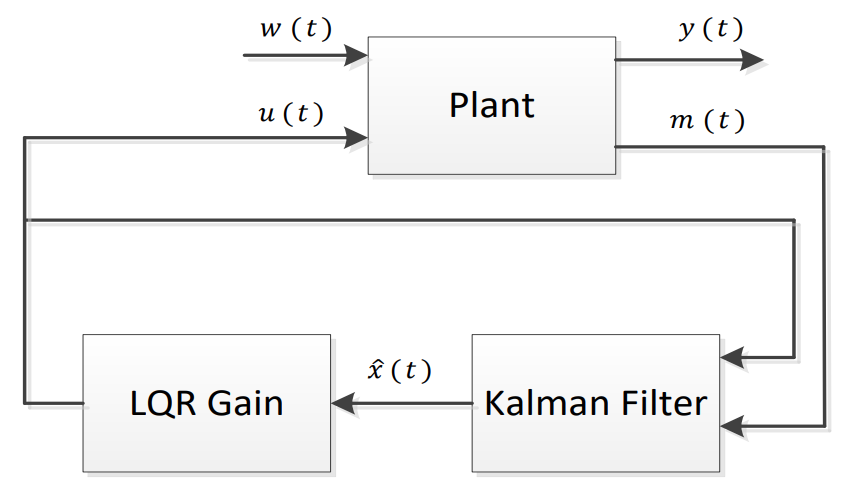
\includegraphics[width=0.6\textwidth]{LQG_control.png}
    \caption{LQG system diagram.}
    \label{fig:LQG_control-png}
\end{figure}

The LQG control is \[
\bm{u}(t) = -K(t)\bm{\hat{x}}(t)
\] that optimizes the cost function \[
J\left( \bm{y}, \bm{u} \right) = \mathbb{E}\left[ \frac{1}{2}\bm{y}^{T}(t_f)H_y\bm{y}(t_f) + \frac{1}{2}\int_0^{t_f}\left\{ \bm{y}^{T}(t)Q_y\bm{y}(t) + \bm{u}^{T}(t)R\bm{u}(t) \right\}dt  \right] 
\]. The Kalman filter will be given by \[
\bm{\hat{\dot{x}}}(t) = \left[  A - G(t)C_m - B_uK(t) \right]\bm{\hat{x}}(t) + G(t)\bm{m}(t)
\].

The solutions will be given by two Riccati equations, one for the control gain \[
\begin{cases}
    \dot{P}(t) = -P(t)A - A^{T}P(t) - Q + P(t)B_uR^{-1}B_u^{T}P(t) \\
    K(t) = R^{-1}B_u^{T}P(t) \\
    P(t_f) = H
\end{cases}
\] and one for the observer \[
\begin{cases}
    \dot{\Sigma}_e(t) = \Sigma_e(t)A^{T} + A\Sigma_e(t) + B_wS_wB_w^{T} - \Sigma_e(t)C_m^{T}S_v^{-1}C_m\Sigma_e(t) \\
    G(t) = \Sigma_e(t)C_m^{T}S_v^{-1} \\
    \Sigma_e(0) = \Sigma_0
\end{cases}
\]. The design of both can be conducted independently.

\section*{Discrete Kalman Filter}

Given a measurement of the form \[
\bm{y} = H\bm{x} + \bm{v}
\] (notice that these are simple vectors, not vector-valued functions), then the estimation that minimizes the estimation error is \[
\bm{\hat{x}} = \left( H^{T}H \right) ^{-1}H^{T}\bm{y}
\]. If we have the confidence matrix $R$ of the noise, defined as \[
R = \mathbb{E}\left[ \bm{v}\bm{v}^{T} \right] 
\] which is a diagonal matrix with the standard deviations of the measurement noise, one can improve the estimation, as in \[
\bm{\hat{x}} = \left( H^{T}R^{-1}H \right) ^{-1}H^{T}R^{-1}\bm{y}
\].

In a linear discrete-time system defined as \[
    \begin{cases}
        \bm{x}_k = F_{k-1}\bm{x}_{k-1} + G_{k-1}\bm{u}_{k-1} + \bm{w}_{k-1} \\
	\bm{y}_k = H_k\bm{x}_k + \bm{v}_k \\
    \end{cases}
\] where $\bm{w}$ and $\bm{v}$ are the model and measurement noises, uncorrelated and with zero mean, the estimation mean can be defined as \[
\bm{\hat{x}}_k^{-} = F\bm{\hat{x}}_{k-1}^{+} + G\bm{u}_{k-1}
\] and its covariance as \[
P_k^{-} = FP_{k-1}^{+}F^{T} + Q
\]. These values are then filtered using \[
\bm{\hat{x}}_k^{+} = \bm{\hat{x}}_k^{-} + K_k\left( \bm{y}_k - H\bm{\hat{x}}_k^{-} \right) 
\] \[
P_k^{+} = \left( I - K_kH \right) P_k^{-}\left( I-K_kH \right) ^{T} + K_kRK_k^{T}
\] in which \[
K_k = P_k^{-}H^{T}\left( HP_k^{-}H^{T} + R \right) ^{-1}
\] and $Q$ and $R$ are the model and measurement noise covariance matrices.

\section*{Lyapunov Stability}

\begin{definition}
Given a system \[
\bm{\dot{x}}(t) = f\left( \bm{x}(t) \right) 
\] and an equilibrium point $\bm{\overline{x}}$ (that is, $\bm{x}(t) = \bm{\overline{x}}\implies\bm{\dot{x}}(t) = 0$), we say this equilibrium point $\bm{\overline{x}}$ is \textbf{stable} if perturbations result in a trajectories that remain in a finite neighborhood of $\bm{\overline{x}}$. $\bm{\overline{x}}$ is said \textbf{asymptotically stable} if it is stable and the trajectories converge to $\bm{\overline{x}}$, that is, given a neighborhood of $\bm{\overline{x}}$ it is true that \[
\lim_{t \to \infty}  \|\bm{x}(t) - \bm{\overline{x}}\|=0
\].
\end{definition}

Lyapunov stability grants us a way to check for stability around an equilibrium point in a non linear system.

\begin{definition}
    (Lyapunov function) Given a system \[
    \bm{\dot{x}}(t) = f\left( \bm{x}(t) \right) 
\] and an equilibrium point $\bm{\overline{x}}$, a function $V:\R^{n}\to \R$ is a \emph{Lyapunov function} on $\bm{\overline{x}}$ if it is \emph{positive-definite} on $\bm{\overline{x}}$.

    (Lyapunov stability) If a Lyapunov function is such that $\frac{\partial V}{\partial t}$ is \emph{negative definite}, then the system is \textbf{stable} on the equilibrium point $\bm{\overline{x}}$. If the Lyapunov function is merely \emph{semi negative-definite}, then is is stable with oscillations around the equilibrium point.
\end{definition}

\begin{note}
    The Lyapunov theorem is a mere \textbf{sufficient condition} for stability.
\end{note}

\subsection*{Gradient Methods}

Given a problem \[
    \underset{x}{\text{min}} f(x)
\], there are two necessary conditions for a vector $\bm{x}^{*}$ to be a local minima:
\begin{itemize}
    \item \[
	    \nabla f(\bm{x}^{*}) = \bm{0}
    \] 
    \item \[
	    \nabla^{2} f(\bm{x}^{*}) >  0
    \] that is, it is \emph{positive definite}.
\end{itemize}
If the second-order derivative of $f$ is positive \emph{semi}-definite, the point must be a saddle point.

The gradient method is an algorithm defined as \[
x_{k+1} = x_k + \alpha_kd_k
\] where \[
d_k = -D_k\nabla f\left( x_k \right) 
\] is the \emph{direction of descent} and is defined by a positive-definite matrix $D_k$, and $\alpha_k$ is the step size.

Two methods exist for defining the direction of descent:
\begin{description}
    \item[Steepest Descent] $D_k = I$
    \item[Newton] $D_k = \left( \nabla ^{2}f\left( x_k \right)  \right) ^{-1}$
\end{description}

\section*{Nonlinear Control}

Both approaches \textbf{define a linear relation between the state variables to simplify the system, reducing its order}.

\subsection*{Variable Structure System}

In this approach to system modeling, the system is allowed to have multiple structure and switch between them. So we can define \[
    \bm{\dot{x}}(t) = \Psi(\bm{x)}(t)\bm{x}(t)
\] \emph{e.g.,} \[
\Psi(x) = \begin{cases}
    -a_1^{2} & \text{if }\dot{x}x>0 \\
    -a_2^2 & \text{if }\dot{x}x<0
\end{cases}
\].

\subsection*{Sliding Model Control (SMC)}

Defines the controller as a VSS. The controller goal is to keep the states in the area where the switching happens, so one does not need to achieve a stable equilibrium point, but just two structures that move the states towards one another. This region of attraction is called the \emph{sliding surface}. This way, one can guarantee that the system is approximately always on the sliding surface.

Given a system \[
\bm{\dot{x}}(t) = f\left( \bm{x}(t), \bm{u}(t) \right) 
\] we want the states to stay in a surface defined by \[
s\left( \bm{x}(t) \right) = 0
\]. A condition on the surface is that it is \emph{locally attractive}, for which we can use Lyapunov theorem to estimate. For example, if we define \[
V\left( \bm{x} \right) = \frac{1}{2}s\left( \bm{x} \right) ^{2}
\] then we know that it suffices to show that \[
\dot{V} = \nabla V \cdot \dot{s} = s\dot{s} < 0
\] in a region around the surface.

To find the controller, we apply the surface restriction to our system, so
\begin{align*}
&s\left( \bm{x}(t) \right) = 0 \\
&\implies \frac{\partial s}{\partial \bm{x}} \bm{\dot{x}}(t) = 0 \\
&\implies \frac{\partial s}{\partial \bm{x}} f\left( \bm{x}(t), \bm{u}(t) \right) = 0
\end{align*}
so this is our goal when designing $\bm{u}(t)$. In a linear setting such as $f(\bm{x}(t),\bm{u}(t)) = A\bm{x}(t) + B\bm{u}(t)$ with a linear surface $s(\bm{x}) = S\bm{x}$, then the controller becomes \[
    \bm{u}(t) = -\left( SB \right) ^{-1}SA\bm{x}(t)
\]. We know that our controller will be of the form \[
\bm{u}(t) = \bm{u}_{eq}(t) + \bm{u}_c(t)
\] where $\bm{u}_eq$ is the controller found when the system is known to stay in the surface, that is, $s(\bm{x}) = 0$ and $\dot{s}(\bm{x}) = 0$.


\subsection*{Synergetic Control}

One bounds the system to move in a limited trajectory in state space defined by \[
    T \dot{\Psi}(\bm{x}) + \Psi(x) = 0
\], so we can design $\bm{u}(t)$ in a continuous manner by solving this equation.

\begin{table}[H]
    \centering
    \caption{SMC vs. Synergetic Control}
    \label{tab:smc-synergetic}
    \begin{tabularx}{0.8\textwidth}{X X}
	\toprule
	SMC & Synergetic Control \\
	\midrule
	Limited set of structures for the system & Limited trajectory? \\
	Extremely robust & Less robust \\
	\bottomrule
    \end{tabularx}
\end{table}

\pagebreak
\section*{Summary}

\subsection*{Canonical forms}

Given \[
    G(s) = \frac{Y(s)}{U(s)} = \frac{b_ms^{m}+\ldots+b_1s + b_0}{s^{n}+a_{n-1}s^{n_1}+\ldots+a_0}\text{, }m<n
\] the controllable and observable forms are dual
\begin{align*}
    A_{observable} = A_{controllable}^{T} ; & B_{observable} = C_{controllable}^{T} \\
    C_{observable} = B_{controllable}^{T} ; & D_{observable} = D_{controllable}
.\end{align*}

\begin{note}
    In a system modeled by a transfer function with cancelling of poles, the controllable form makes a controllable system but not observable, while the observable makes the opposite.
\end{note}

The Jordan (or diagonal) canonical form is based on the fractions expansion of $G(s)$, so \[
    G(s) = \frac{Y(s)}{U(s)} = \sum_{i=1}^{n} \frac{c_i}{s-s_i}
\], which becomes
\begin{align*}
    A =
    \begin{bmatrix}
	s_1 & 0 & \ldots & 0 \\
	0 & s_2 & \ldots & 0 \\
	\vdots & & \ddots & \vdots \\
	0 & \ldots & 0 & s_n
	\end{bmatrix} \\
	B = I ; C = \begin{bmatrix} c_1 & \ldots & c_n \end{bmatrix} 
.\end{align*}

\subsection*{Pole Placement}

Controllability and observability are dual conditions.

\begin{definition}
    (Controllability) A system is said to be \textbf{controllable} if it is possible, through an unbounded input, to take it from any initial state to any other state in finite time. It is \textbf{completely state controllable} if this is true for every state.

    \textbf{A system is controllable $\iff rank\left( W_c \right) = n$}
\end{definition}

\begin{definition}
    (Observability) A system is said to be \textbf{observable} if it is possible, through a limited observation of the output $\bm{y}(t)$, to determine the state $x_i(t_0)$. It is \textbf{completely observable} if this is true for every state.

    \textbf{A system is observable $\iff rank\left( W_o \right) = n$}
\end{definition}

\begin{note}
    First step in the design of a controller through pole placement is \textbf{always to check controllability}.
\end{note}

Approaches to the design of $K : \bm{u}(t) = -K\bm{}(t)$ provides us with a system with the desired poles $\mu_1,\ldots,\mu_n$.

\begin{description}
    \item[Direct Substitution] Solve \[
	\prod_{i=1}^{n} \left(  \lambda - \mu_i\right) = det(\lambda I - A + BK)
    \] by matching the coefficients of like powers of $\lambda$.
    \item[Transformation Matrix] Define a transformation matrix $T = MW$ where $M=W_c$ and \[
    W =
    \begin{bmatrix}
	a_{n-1} & a_{n-2} & \ldots & a_1 & 1 \\
	a_{n-2} & a_{n-3} & \ldots & 1 & 0 \\
	\vdots & \vdots & \vdots & \ddots & \vdots \\
	1 & 0 & \ldots & 0 & 0 \\
    \end{bmatrix} 
    \], then, we subtract the open-loop characteristic equation coefficients from the desired ones, that is, for \[
    det(\lambda I - A) = \lambda^{n} + a_1\lambda^{n-1} + \ldots + a_{n-1}\lambda + a_n
    \] and \[
    \prod_{i=1}^{n} \left(  \lambda - \mu_i\right) = \lambda^{n} + \alpha_1\lambda^{n-1} + \ldots + \alpha_{n-1}\lambda + \alpha_n
    \] we compute \[
    K = \begin{bmatrix} \alpha_n - a_n & \ldots & \alpha_1 - a_1 \end{bmatrix} T^{-1}
    \].
    \item[Ackermann's Formula] We can design $K$ through through \[
	    K = \begin{bmatrix} 0 & \ldots & 0 & 1 \end{bmatrix} W_c^{-1}\Phi(A)
    \], where \[
	\Phi(A) = A^{n} + \alpha_1A^{n-1} + \ldots + \alpha_{n-1}A + \alpha_nI
	\] is the desired characteristic equation evaluated at $A$.
\end{description}

\subsection*{State Observer}

\begin{note}
    The first step in designing an observer is to check for the system's observability.
\end{note}

An observer has the form \[
\begin{cases}
    \dot{\bm{\hat{x}}}(t) = A\bm{\hat{x}}(t) + B\bm{u}(t) + L\left( \bm{y}(t) - \bm{\hat{y}}(t)\right) \\
    \bm{\hat{y}}(t) = C\bm{\hat{x}}(t) + D\bm{u}(t)
\end{cases}
\] and we \textbf{design the matrix $L$ through pole placement} on the error equation, that is, if $\bm{e}(t) = \bm{x}(t) - \bm{\hat{x}}(t)$, then \[
\bm{\dot{e}}(t) = \left( A-LC \right) \left( \bm{x}(t) - \bm{\hat{x}}(t) \right) 
\], so we just need to place the eigenvalues of $A-LC$ on the LHP.

\subsection*{LQR}

Cost function is defined as \[
    J(\bm{x}, \bm{u}) = \frac{1}{2}\bm{y}(t_f)^{T}H_y \bm{y}(t_f) + \frac{1}{2}\int_0^{t_f}\left[ \bm{y}(t)^{T}Q_y \bm{y}(t)  +  \bm{u}(t)^{T}R\bm{u}(t) \right] dt
\]. Use this to find $H$, $Q$ and $R$;

The optimal controller for this formulation is \[
K = R^{-1}B^{T}P
\], so we must define $P$.

 \begin{description}
    \item[Hamiltonian] The hamiltonian matrix is defined as \[
H_a = \begin{bmatrix} A & -BR^{-1}B^{T} \\ -Q & -A^{T} \end{bmatrix}
    \] and we can find $P$ through the positive eigenvalue $\lambda_p$ of this matrix, as \[
    H\begin{bmatrix} \Psi_{11} \\ \Psi_{21} \end{bmatrix} = \lambda_p\begin{bmatrix} \Psi_{11} \\ \Psi_{21} \end{bmatrix}
    \] and then \[
    P = \Psi_{21}\Psi_{12}^{-1}
    \].
    \item[Riccati] The Riccati equation gives us \[
    \dot{P}(t) + P(t)A + A^{T}P(t) + Q - P(t)BR^{-1}B^{T}P(t) = 0
    \] with final condition \[
    P(t_f) = H
    \], which is solvable in steady state. \textbf{The positive definite solution of $P$ must be chosen}.
\end{description}

The optimal cost can also be calculated through \[
    J = \frac{1}{2}\bm{x}(0)^{T}P(0)\bm{x}(0)
\].

\subsection*{Kalman Filter}

Is a stochastic estimator that minimizes \[
J = \mathbb{E}\left[ \bm{e}^{T}(t)\bm{e}(t) \right]
\].

The estimator has form \[
\dot{\bm{\hat{x}}}(t) = A\bm{\hat{x}}(t) + B_u\bm{u}(t) + G(t)\left[ \bm{m}(t) - C_m\bm{\hat{x}}(t) \right] 
\] and the gain matrix $G(t)$ of the estimator can be determined as \[
G(t) = \Sigma_e(t)C_m^{T}S_v^{-1}
\], so we need to determine $\Sigma_e$, which can be done similarly as the LQR problem for the $P$ matrix. The major difference is that in the hamiltonian approach, \textbf{the positive eigenvalue must be chosen}.

\subsection*{LQG}

Combines LQR and Kalman Filter. The design of both components can be handled independently.

\subsection*{Discrete Kalman Filter}

In a discrete-time system defined as \[
    \begin{cases}
        \bm{x}_k = F_{k-1}\bm{x}_{k-1} + G_{k-1}\bm{u}_{k-1} + \bm{w}_{k-1} \\
	\bm{y}_k = H_k\bm{x}_k + \bm{v}_k \\
    \end{cases}
\], the Kalman Filter can be applied in an estimation-filtering approach, in which each discrete step is performed as follows:
\begin{enumerate}
    \item Estimate the state mean value $\bm{\hat{x}}_k^{-} = F\bm{\hat{x}}_{k-1}^{+} + G\bm{u}_{k-1}$;
    \item Estimate state covariance $P_k^{-} = FP_{k-1}^{+}F^{T} + Q$ with the model noise covariance matrix $Q$;
    \item Compute the Kalman Gain $K_k = P_k^{-}H^{T}\left( HP_k^{-}H^{T} + R \right) ^{-1}$ with the measurement noise covariance matrix $R$;
    \item Filter the estimation of the state mean value $\bm{\hat{x}}_k^{+} = \bm{\hat{x}}_k^{-} + K_k\left( \bm{y}_k - H\bm{\hat{x}}_k^{-} \right)$ and of the state covariance $P_k^{+} = \left( I - K_kH \right) P_k^{-}\left( I-K_kH \right) ^{T} + K_kRK_k^{T}$.
\end{enumerate}

\subsection*{Gradient Methods}

Given a problem of the form \[
    \underset{x}{\text{min}} f(x)
\], there are two conditions for a vector $\bm{x}^{*}$ to be a local minima:
\begin{itemize}
    \item $\nabla f(\bm{x}^{*}) = \bm{0}$ \\
    \item $\nabla ^2f(\bm{x}^{*}) > 0$ \\
.\end{itemize}

The gradient method converges (for sufficiently small $\alpha$ value) to a local minima and is defined as \[
x_{k+1} = x_k + \alpha_kd_k
\] where \[
d_k = -D_k\nabla f\left( x_k \right) 
\] is the \emph{direction of descent} and is defined by a positive-definite matrix $D_k$, and $\alpha_k$ is the step size.

Two methods exist for defining the direction of descent:
\begin{description}
    \item[Steepest Descent] $D_k = I$
    \item[Newton] $D_k = \left( \nabla ^{2}f\left( x_k \right)  \right) ^{-1}$
\end{description}

\subsection*{Lyapunov Stability}

An equilibrium point $\bm{\overline{x}} : \bm{x}(t)=\bm{\overline{x}}\implies\bm{\dot{x}}(t) = 0$ is said to be \textbf{Lyapunov stable} if the trajectories from initial conditions in a neighborhood of $\bm{\overline{x}}$ stay in a neighborhood of $\bm{\overline{x}}$. It is \textbf{asymptotically stable} if it is Lyapunov stable and \[
\lim_{t \to \infty} \|\bm{x}(t)-\bm{\overline{x}}\|=0
\].

Given a system $\bm{\dot{x}}(t) = f\left( \bm{x}(t) \right) $ with an equilibrium point $\bm{\overline{x}}$, then a function $V:\R^{n}\to \R$ such that
\begin{align*}
    &V(\bm{x}) = 0 \iff \bm{x} = \bm{\overline{x}} \\
    &V(X) > 0 \iff \bm{x} \neq \bm{\overline{x}} \\
    &\dot{V}(\bm{x}) = \nabla V \cdot f(\bm{x}) \le 0 \forall \bm{x}\neq \bm{\overline{x}} \\
\end{align*}
is a \textbf{Lyapunov function} and the equilibrium point is \textbf{stable}. If $\dot{V}(\bm{x}) <0 \forall \bm{x}\neq \bm{\overline{x}}$, then the equilibrium point is \textbf{asymptotically stable}.

\subsection*{Nonlinear control}

Given a surface $\Psi(\bm{x})$ on the state space, we define our controller such that this surface is \emph{locally attractive}. That is, our controller $\bm{u}$ must be such that, given a Lyapunov function over the surface \[
    V(\Psi(\bm{x})) = \frac{1}{2}\Psi^2(\bm{x})
\] we have that \[
\dot{V}(\bm{x}) < 0
\], which means that this surface is asymptotically stable.

\begin{table}[H]
    \centering
    \caption{SMC vs. Synergetic Control}
    \label{tab:smc-synergetic}
    \begin{tabularx}{0.8\textwidth}{X X}
	\toprule
	SMC & Synergetic Control \\
	\midrule
	$\Psi(\bm{x}) = 0 $ & $T \dot{\Psi}(\bm{x}) + \Psi(x) = 0$ \\
	Discontinuous solution, VSS & Continuous solution \\
	Extremely robust & Less robust \\
	\bottomrule
    \end{tabularx}
\end{table}

\end{document}
